\documentclass[12pt]{article}
\setlength{\oddsidemargin}{0in}
\setlength{\evensidemargin}{0in}
\setlength{\textwidth}{6.5in}
\setlength{\parindent}{0in}
\setlength{\parskip}{\baselineskip}
\setlength{\headheight}{43pt}

\usepackage{amsmath,amsfonts,amssymb}
\usepackage{graphicx}
\usepackage{fancyhdr}
\usepackage{enumerate}
\usepackage{forest}
\usepackage{float}
\usepackage{cprotect}
\usepackage{listings}
\usepackage{tikz}
\usetikzlibrary{arrows,backgrounds,calc}
\pagestyle{fancy}

\lstset{
    language=python,
    numbers=left,
    tabsize=2,
    showstringspaces=false,
    showspaces=false,
    numberstyle=\tiny,
    xleftmargin=4em,
    resetmargins=true,
}

\pgfdeclarelayer{background}
\pgfsetlayers{background,main}
\newcommand{\convexpath}[2]{
[   
    create hullnodes/.code={
        \global\edef\namelist{#1}
        \foreach [count=\counter] \nodename in \namelist {
            \global\edef\numberofnodes{\counter}
            \node at (\nodename) [draw=none,name=hullnode\counter] {};
        }
        \node at (hullnode\numberofnodes) [name=hullnode0,draw=none] {};
        \pgfmathtruncatemacro\lastnumber{\numberofnodes+1}
        \node at (hullnode1) [name=hullnode\lastnumber,draw=none] {};
    },
    create hullnodes
]
($(hullnode1)!#2!-90:(hullnode0)$)
\foreach [
    evaluate=\currentnode as \previousnode using \currentnode-1,
    evaluate=\currentnode as \nextnode using \currentnode+1
    ] \currentnode in {1,...,\numberofnodes} {
  let
    \p1 = ($(hullnode\currentnode)!#2!-90:(hullnode\previousnode)$),
    \p2 = ($(hullnode\currentnode)!#2!90:(hullnode\nextnode)$),
    \p3 = ($(\p1) - (hullnode\currentnode)$),
    \n1 = {atan2(\y3,\x3)},
    \p4 = ($(\p2) - (hullnode\currentnode)$),
    \n2 = {atan2(\y4,\x4)},
    \n{delta} = {-Mod(\n1-\n2,360)}
  in 
    {-- (\p1) arc[start angle=\n1, delta angle=\n{delta}, radius=#2] -- (\p2)}
}
-- cycle
}

\begin{document}

\lhead{{\bf Grant Baker (07/23) \\ Samuel Cuthbertson (06/16) \\ Connor Hudson (05/07)} }
\rhead{{\bf CSCI 3104 Algorithms\\ Problem Set 8\\ Spring 2017, CU-Boulder}}
\renewcommand{\headrulewidth}{0.5pt}
\vspace{-3mm}
\begin{enumerate}

	
    % PROBLEM 1
     \item \textit{(30 pts total) On an overnight camping trip in the Forbidden Forest near the Hogwarts School of Witchcraft and Wizardry, you and your 
wizard friends Ron and Hermione are woken from a restless sleep by a scream. Crawling out of your tent to investigate, you see a terrified young wizard 
stumble out of the woods, covered in blood and clutching a crumpled piece of paper to her chest. Reaching your tent, she gasps “Get out... while... you...”, 
thrusts the paper into your hands and falls to the ground, dead.}
     
     \textit{Looking at the crumpled paper, you recognize a map of the forest, drawn as an undirected graph, where vertices represent landmarks in the forest, 
and edges represent trails between those landmarks. (Trails start and end at landmarks and do not cross.) Coincidentally, you recognize one of the vertices as 
your current location; several vertices on the boundary of the map are labeled EXIT.}
     
     \textit{On closer examination, you notice that someone (perhaps the dead wizard) has written a real number between 0 and 1 next to each vertex and each 
edge. A scrawled note on map's reverse side indicates that these numbers give the probability of encountering a deadly Dementor along the corresponding trail 
or at the corresponding landmark. The note warns that stepping off the marked trails will surely result in death.}
     
     \textit{You glance down at the corpse at your feet. Her death certainly looked painful. On closer examination, you realize that the wizard is not dead at 
all, or rather, is turning into a Dementor who will surely devour you. After burning the wizard's body, you wisely decide to leave the forest immediately.}

    \begin{enumerate}
        \item \textit{Give a (small!) example G such that the path from your current location to the EXIT node that minimizes the expected number of 
encountered Dementors is different from the path that minimizes the probability of encountering any Dementors at all. Explain why, in general, these two 
criteria lead to different answers.}\\
        
        Let $D$ be a random variable corresponding to the number of dementors encountered along a path $Q$. The expected number of dementors along a path is 
given by 
        \[
            E[D] = \sum_{q \in Q} p_q
        \]
        where $e$ is an edge in the path $Q$, and $p_e$ is the corresponding probability of encountering a dementor along that path. The probability of 
encountering a dementor at any point along the path is given by 
        \begin{align*}
            P\{D \geq 1\} &= 1 - P\{D = 0\}\\
            &= 1 - P\{\text{don't encounter dementor on each edge or node}\}\\
            &= 1 - \prod_{q \in Q} P\{\text{don't encounter dementor on edge or node } q\}\\
            &= 1 - \prod_{q \in Q} (1 - p_q)
        \end{align*}
        since the only event in which $D=0$ is the event where no dementors are encountered on each edge taken, for which each edge has probability $(1 - 
p_e)$ and we assume independence of these events.\\
        
        \begin{center}
            \begin{tikzpicture}
                \node[circle, very thick, draw] (S) at (0,0) {S};
                \node[circle, very thick, draw] (V1) at (2,1) {V};
                \node[circle, very thick, draw] (V2) at (2,-1) {V};
                \node[circle, very thick, draw] (E) at (4,0) {E};
                
                \node[above of = V1] {0.0};
                \node[below of = V2] {0.0};
                
                \draw (S) -- node[circle, above left] {$0.8$} (V1);
                \draw (S) -- node[circle, below left] {$0.5$} (V2);
                \draw (V2) -- node[circle, below right] {$0.5$} (E);
                \draw (V1) -- node[circle, above right] {$0.1$} (E);
            \end{tikzpicture}
        \end{center}
        
        The expected number of dementors along the top path is $0.9$, and along the bottom path it is $1$. The minimum expected number of dementors is along 
the top path.\\
        
        The probabililty of encountering a dementor along the top path is $0.82$, and along the bottom path it is $0.75$. The minimum probability is along the 
bottom path, different from the other criterion.\\
        
        In general, these two criteria lead to different answers, in a broad sense, because the expectation considers encountering more than one dementor and 
the probability does not. More specifically, the criteria are different because we can think about the number of dementors encountered $D$ as a random 
variable:
        \[
            D = \sum \text{Bernoulli}(p_i)
        \]
        where $p_i$ are the probabilities along each edge and node. Then the two criteria can be written as
        \begin{align*}
            E[D] &= \sum p_i\\
            P\{D \geq 1\} &= 1 - \prod (1-p_i)
        \end{align*}
        which in general have different values.\\
        
        
        \item \textit{Describe and analyze an efficient algorithm to find a path from your current location to an arbitrary EXIT node, such that the total 
expected number of Dementors encountered along the path is as small as possible. Be sure to account for both the vertex probabilities and the edge 
probabilities.}
        
        \textit{Dumbledore's hint: This is clearly an SSSP problem, but you must identify how to reduce the input G to a form that can be solved by SSSP. 
Remember to include the cost of this transformation in your running-time analysis.}\\
        
        Since the expected number of Dementors is precisely the sum of the probabilities of encountering a dementor along each edge on the path and on each 
node on the path, we can adapt an SSSP algorithm, specifically Dijkstra (since probabilities are nonnegative), to account for weight at nodes when examining 
if a node is tense and relaxing it.
         
        \begin{small}
        \begin{verbatim}
escapeForest(G, s):
    dist(s) = P(s)
    pred(s) = NULL
    for v in G, v != s:
        dist(v) = INF
        pred(v) = NULL
    Q = emptySet()     // fibonacci min-heap
    
    Q.add(s)
    while Q.notEmpty():
        u = Q.get()
        for all edges (u,v):
            if dist(v) > dist(u) + P(v) + P(u,v):   // calculating tenseness
                dist(v) = dist(u) + P(v) + P(u,v)
                pred(v) = u
                Q.add(v)
        \end{verbatim}
        \end{small}
    % u = e
    % path = {e}
    % while u != s:
    %     u = pred(u)
    %     appendTo(path, u)
        
    % return path
        
        This algorithm is precisely the SSSP algorithm given in lecture notes, but with the distance updated to be the probability $p_i$ and takes into 
consideration the probability at vertices.\\
        
        Its runtime is exactly the same as SSSP, since the extra computations required to compute tenseness are constant time, so if we use Dijkstra with a 
Fibonacci min-heap we have $O(E + V\log V)$.\\
         
        
        \item \textit{Describe and analyze an efficient algorithm to find a path from your current location to an arbitrary EXIT node, such that the 
probability of encountering any Dementors at all is minimized.}\\
        
        Again, this is precisely SSSP but instead of an additive distance of the probabilies we must substitute a multiplicative one that takes into 
consideration to what event each probability corresponds. More precisely, our weight will be
        \[
        W[Q] = 1 - \prod_{q\in Q} (1 - p_q)
        \]
        where $Q$ is the path, $p_q$ corresponds to the probability at node or edge $q$, and $W$ is the weight. If we attempt to minimize this like a distance 
with SSSP, we will get the correct result.
        
        \begin{small}
        \begin{verbatim}
escapeForest(G, s):
    dist(s) = P(s)
    pred(s) = NULL
    for v in G, v != s:
        dist(v) = INF
        pred(v) = NULL
    Q = emptySet()     // fibonacci min-heap
    
    Q.add(s)
    while Q.notEmpty():
        u = Q.get()
        for all edges (u,v):
            if dist(v) > 1 - (1 - dist(u))*(1 - P(u,v))*(1 - P(v)):
                dist(v) = 1 - (1 - dist(u))*(1 - P(u,v))*(1 - P(v))
                pred(v) = u
                Q.add(v)
        \end{verbatim}
        \end{small}
                
    % u = e
    % path = {e}
    % while u != s:
    %     u = pred(u)
    %     appendTo(path, u)
        
    % return path
        
        Again, this is the SSSP algorithm in the lecture notes with the criterion for tenseness relying on probability, the theory for which is described in 
part (a).\\
        
        The runtime of this algorithm is again the runtime for the SSSP algorithm, so if we use Dijkstra with a Fibonacci min-heap we have $O(E+V\log V)$.
         
    \end{enumerate}
    
    
    % PROBLEM 2
    \newpage
    \item \textit{(30 pts total) In a late-night algorithms study session, you and Draco Malfoy are arguing about the conditions under which a minimum 
spanning tree is unique. You agree that if all edges in $G$ have unique weights the MST is also unique, but you disagree about how to relax this assumption. 
Let $w(e)$ be a function that returns the weight of some $e \in E$.}
    \begin{enumerate}
         \item \textit{Give an example of a (small!) weighted graph that has both a unique MST and some pair of edges $e$ and $e'$ such that $w(e) = w(e') = 
x$.}
         \begin{center}
            \begin{tikzpicture}
            
                \node[circle, minimum size=.25, draw, fill] (B) at (0,0) {};
                \node[circle, minimum size=.25, draw, fill] (L) at (2,1) {};
                \node[circle, minimum size=.25, draw, fill] (R) at (2,-1) {};
                \node[circle, minimum size=.25, draw, fill] (T) at (4,0) {};
                
                \draw (B) -- node[above left, circle] {4} (L);
                \draw [line width=2pt] (B) -- node[below left, circle] {1} (R);
                \draw [line width=2pt] (R) -- node[below right, circle] {3} (T);
                \draw [line width=2pt] (L) -- node[above right, circle] {1} (T);
                
            \end{tikzpicture}
         \end{center}
         
         The above graph has a unique MST as running Prim's algorithm on any node will yield the same tree, even though there are two edges of weight 1.\\
         
         \item \textit{Malfoy claims that the following is true. Prove via (small!) counter examples that it is false.}
         
         \textit{Malfoy's Claim: $G$ has a unique MST if and only if (i) for any partition of the vertices of $G$ into two subsets, the minimum-weight edge 
with one endpoint in each subset is unique, and (ii) the maximum-weight edge in any cycle of $G$ is unique.}
         
         \begin{center}
            \begin{tikzpicture}
            
                \node[circle, minimum size=.25, draw, fill] (B) at (0,0) {};
                \node[circle, minimum size=.25, draw, fill] (L) at (2,1) {};
                \node[circle, minimum size=.25, draw, fill] (R) at (2,-1) {};
                \node[circle, minimum size=.25, draw, fill] (T) at (4,0) {};
                
                \draw (B) -- node[above left,circle] {\:4} (L);
                \draw (B) -- node[above, pos=0.6] {4} (T);
                \draw [line width=2pt] (B) -- node[below left, circle] {1} (R);
                \draw [line width=2pt] (R) -- node[below right, circle] {3} (T);
                \draw [line width=2pt] (L) -- node[above right, circle] {1} (T);
                
                \fill[red,opacity=0.3] \convexpath{B,L}{18pt};
                \fill[blue,opacity=0.3] \convexpath{R,T}{18pt};
                
            \end{tikzpicture}
         \end{center}
         
         The above graph has a unique MST, as running Prim's algorithm on any node will yield the same tree. Additionally, the minimum weight edge with one 
endpoint in each subset of red and blue is not unique as there are two edges of weight 1 which satisfy the constraints. Finally, the cycle of edges 4-4-1 has 
two edges that tie for maximum weight.
         
         \newpage
         \item \textit{Malfoy now demands that you produce the correct relaxed condition, which you claim is the following. Prove that you are correct.}
         
         \textit{Your Claim: an edge-weighted graph $G$ has a unique MST $T_{mst}$ if and only if the following conditions hold:} \\
         \textit{(i) for any bipartition of the vertices induced by removing some edge $e \in T_{mst}$, the minimum-weight edge with one endpoint in each 
subset is unique, and \\ (ii) the maximum-weight edge of any cycle constructed by adding one edge $f$ to $T_{mst}$, where $f \notin T_{mst}$, is unique.}
         
         \textit{Dumbledore's hint: Note that for any spanning tree $T$ on $G$, removing some edge $e \in T$ induces a bipartition of the vertices. Consider 
the edges that span this cut.}\\
         
         There are four proofs here, proving bidirectionally both (i) and (ii), each done by contraposition.\\
         
         Claim: If $G$ has a unique MST $T_{mst}$, then any bipartition of the vertices induced by removing some edge $e \in T_{mst}$, the minimum-weight edge 
with one endpoint in each subset is unique.\\
         
         Proof: Suppose $G$ has a unique MST $T_{mst}$. Now suppose we remove an edge $e \in T_{mst}$. $e$ is the minimum-weight edge between the two 
partitions, because if there was another edge spanning the partitions with a lower weight it would have been included in the MST rather than $e$.
         
         By way of contradiction, suppose $e$ is not unique. Then there is another edge $\hat{e}$ with the same weight as $e$. Now if $\hat{e}$ is added to 
$T_{mst} \backslash \{e\}$, the result $\hat{T}_{mst}$ is a new MST since $e$ and $\hat{e}$ have the same weight. This shows that the $MST$ is not unique, 
contradicting our assumption of uniqueness of $T_{mst}$.
         
         Therefore, the minimum-weight edge $e$ is unique.\\
         
         Claim: If for any bipartition of the vertices induced by removing $e \in T_{mst}$, the minimum-weight edge with one endpoint in each set is unique, 
then the MST $T_{mst}$ is unique.\\
         
         Proof: Suppose not, by way of contraposition. Then there is at least one $e$ in $T_{mst}$ that can be removed and replaced with another edge 
$\hat{e}$ to produce a different MST $\hat{T}_{mst}$.
         
         Create the partition of the vertices by removing $e$ from $T_{mst}$. Since $e \in T_{mst}$, then $e$ is the minimum-weight edge between partitions. 
But since $\hat{e}$ can be added to create another MST, then the weight of $\hat{e}$ and $e$ must be the same (otherwise $\hat{T}_{mst}$ would not exist).
         
         This contradicts the assumption of the uniqueness of $e$, so therefore the MST $T_{mst}$ is unique.\\
         
         Claim: If $G$ has a unique MST $T_{mst}$, the the maximum-weight edge of any cycle constructed by adding one edge $f$ to $T_{mst}$, where $f \not \in 
T_{mst}$, is unique.\\
         
         Proof: Suppose not. Then, we can add an edge $f$ to $T_{mst}$ to create a cycle $C$ where the weight of $f$ is $\max \{c \in C \hspace{6pt} | 
\hspace{6pt} c \in T_{mst}\}$. Note that the weight of $f$ cannot be lower than this or $T_{mst}$ would not be a MST.
         
         Then the max-weight edge of this cycle is not unique, since it is both $f$ and the max of the rest of the edges, called $e$. Note that $e \in 
T_{mst}$.
         
         Then, suppose we remove $e$ from $T_{mst}$ and add $f$ to $T_{mst}$. Since we still have connectedness within the cycle $C$, the resulting set $U$ is 
a spanning tree. Since the weight of $f$ and $e$ are equal, then $U$ is a different MST from $T_{mst}$.
         
         This contradicts the assumption that $T_{mst}$ is unique, so the max weight edge $f$ in the cycle $C$ is unique.\\
         
         Claim: If the maximum-weight edge of any cycle constructed by adding one edge $f$ to $T_{mst}$, where $f \not \in T_{mst}$, is unique, then the MST 
$T_{mst}$ is unique.\\
         
         Proof: Suppose not. Then there is at least one edge $e \in T_{mst}$ that we can replace with a different edge $f \not \in T_{mst}$ to create a new 
MST $\hat{T}_{mst}$. Since they are both MSTs, the weights of $e$ and $f$ are the same. Now construct a cycle $C$ that includes both $e$ and $f$.
         
         Since $e$ and $f$ are in MSTs, but are interchangable, we know that $e$ and $f$ have the maximum weights in the cycle. Otherwise, one of them would 
always not be included in an MST. But they are the same maximum weight, and thus there is not a unique maximum to the cycle $C$.
         
         This contradicts our assumption that the max-weight edge of the cycle is unique, so the MST $T_{mst}$ is unique.\\
        
         \newpage
         
         \item \textit{Describe and analyze an algorithm that will determine whether an input graph $G$ has a unique MST in (effectively) $O(E \log V )$ 
time.\footnote{Collaboration and assistance from Luke Meszar}} 
         
         An efficient way to solve this would be to make a min heap of all the edges, exactly like Kruskal's algorithm, only have each edge be part of a 
tuple. Have the other value in the tuple be a binary (0 by default) value. This would take $O(E \log V)$, as generating the tuples would run in $O(E)$ time 
while generating the min-heap dominates with $O(E \log V)$ time.
         
         Next, generate a MST in the same way Kruskal's generates a MST, only change the second value in each edge to 1 when it is used in the MST. This is 
(effectively) $O(1)$, as it uses union-find which is explained in the lecture notes.
         
         Finally, generate a new min-heap using the updated edges, and run Kruskal's algorithm, only with a modified version of Union-Find which checks if 
there is a tie between two edges (two edges of the same weight that are both in the union) where only one has been in the MST before (only one has a 1 in the 
second value of the tuple). If, at any point, such a pair is encountered, then the graph does not have a unique MST. This is also effectively $O(E \log V)$, 
since generating a min-heap is the expensive operation here. Note that using union-find on two sets, as would be done to check for a tie, is the equivalent of 
$2*O(1) = O(1)$.
         
         All the runtimes combined still come out to $O(E \log V)$, all of which comes from generating the min-heaps of edges.
         
        %  \textsf{CAN I USE THE LIL PROOF BOX? DID I DO IT RIGHT? :O -S}
    
    % PROBLEM 3
    \newpage
    \end{enumerate}
    \item \textit{(20 pts) Let $G$ be a graph, $w$ be a weight function for its edges, and $T$ be one of its minimum spanning trees. Now, suppose that we 
modify $G$ slightly by decreasing the weight of exactly one of the edges in $T$, producing a new graph $G'$. Prove that $T$ is also a minimum spanning tree 
for $G'$. More formally, let the edge choice be denoted $(x, y) \in T$, $k$ be a positive number, and define the weight function $w'$ by}
    \begin{align*}
        w'(u,v) = 
        \begin{cases}
            w(u,v)      & \text{if} (u,v) \neq (x,y)\\
            w(x,y) - k  & \text{if} (u,v) = (x,y)
        \end{cases}
    \end{align*}
    
    \textit{Prove that $T$ is a minimum spanning tree for $G'$ , whose edge weights are given by $w'$.}
    
    If $T$ is a spanning tree on $G$, then by definition $\sum_{e \in T} w(e)$ is minimized. If we \textit{decrease} the weight of one of the edges in $T$ by 
some value $k$ and modify no other edge weights in the graph, the total weight $w(T)$ of the tree must also be the minimum weight for the graph. \\
    
    Also note that since we have modified $G$ in no other way besides modifying the edge function, $T$ is still a spanning tree for $G'$. Since $w(T)$ is 
minimized and $T$ is a spanning tree on $G'$, by definition $T$ is a minimum spanning tree.
    
    
    % PROBLEM 4
    \newpage
    \item \textit{(20 pts) Professor Snape gives you the following unweighted graph and asks you to construct a weight function w on the edges, using positive 
integer weights only, such that the following conditions are true regarding minimum spanning trees and single-source shortest path trees: }\textit{The MST is 
distinct from any of the seven SSSP trees. }\textit{The order in which Jarn\'{i}k/Prim's algorithm adds the safe edges is different from the order in which 
Kruskal's algorithm adds them. }\textit{Bor\.{u}vka's algorithm takes at least two rounds to construct the MST. }
    \textit{Justify your solution by (i) giving the edges weights, (ii) showing the corresponding MST and all the SSSP trees, and (iii) giving the order in 
which edges are added by each of the three algorithms. (For Bor\.{u}vka's algorithm, be sure to denote which edges are added simultaneously in a single 
round.)}
    \begin{center}
        \begin{minipage}{0.4\textwidth}
            \begin{center}
                \begin{tikzpicture}[scale=.85]
                
                    \node[circle, ultra thick, draw, fill=orange!80] (a) at (0,2) {\bf a};
                    \node[circle, ultra thick, draw, fill=orange!80] (b) at (2,4) {\bf b}; \node[circle, ultra thick, draw, fill=orange!80] (c) at (2,0) {\bf 
c}; \node[circle, ultra thick, draw, fill=orange!80] (d) at (4,2) {\bf d}; \node[circle, ultra thick, draw, fill=orange!80] (e) at (6,4) {\bf e}; 
\node[circle, ultra thick, draw, fill=orange!80] (f) at (8,2) {\bf f}; \node[circle, ultra thick, draw, fill=orange!80] (g) at (6,0) {\bf g}; 
                    
                    \draw[ultra thick, blue] (a) -- node[above, sloped] {$3$} (b);
                    \draw[ultra thick, blue] (a) -- node[below, sloped] {$5$} (c);
                    \draw[ultra thick] (b) -- node[right] {$15$} (c);
                    \draw[ultra thick] (b) -- node[above, sloped] {$13$} (d);
                    \draw[ultra thick, blue] (b) -- node[above, sloped] {$7$} (e);
                    \draw[ultra thick] (c) -- node[below, sloped] {$21$} (d);
                    \draw[ultra thick] (c) -- node[below, sloped] {$25$} (g);
                    \draw[ultra thick, blue] (d) -- node[above, sloped] {$9$} (e);
                    \draw[ultra thick, blue] (d) -- node[below, sloped] {$1$} (g);
                    \draw[ultra thick] (e) -- node[above, sloped] {$23$} (f);
                    \draw[ultra thick] (e) -- node[right] {$29$} (g);
                    \draw[ultra thick, blue] (g) -- node[below, sloped] {$19$} (f);
                    
                \end{tikzpicture}
            \end{center}
        \end{minipage}
        \hfill
        \begin{minipage}{0.4\textwidth}
            \begin{center}
                Our graph, with the MST shown composed of the edges highlighted in blue.
            \end{center}
        \end{minipage}
                \begin{minipage}{0.4\textwidth}
            \begin{center}
                \begin{tikzpicture}[scale=.85]
                
                    \node[circle, ultra thick, draw, fill=orange!80] (a) at (0,2) {\bf a};
                    \node[circle, ultra thick, draw, fill=orange!80] (b) at (2,4) {\bf b}; \node[circle, ultra thick, draw, fill=orange!80] (c) at (2,0) {\bf 
c}; \node[circle, ultra thick, draw, fill=orange!80] (d) at (4,2) {\bf d}; \node[circle, ultra thick, draw, fill=orange!80] (e) at (6,4) {\bf e}; 
\node[circle, ultra thick, draw, fill=orange!80] (f) at (8,2) {\bf f}; \node[circle, ultra thick, draw, fill=orange!80] (g) at (6,0) {\bf g}; 
                    
                    \draw[ultra thick, blue] (a) -- node[above, sloped] {$4$} (b);
                    \draw[ultra thick, blue] (a) -- node[below, sloped] {$5$} (c);
                    \draw[ultra thick, blue] (b) -- node[above, sloped] {$3$} (e);
                    \draw[ultra thick, blue] (d) -- node[above, sloped] {$2$} (e);
                    \draw[ultra thick, blue] (d) -- node[below, sloped] {$1$} (g);
                    \draw[ultra thick, blue] (g) -- node[below, sloped] {$6$} (f);
                    
                \end{tikzpicture}
            \end{center}
        \end{minipage}
        \hfill
        \begin{minipage}{0.4\textwidth}
            \begin{center}
                Our MST, with the edges numbered by the order they are added by Prim's algorithm. Note: We assumed Prim's would start with the mimimum weight 
edge. 
            \end{center}
        \end{minipage}
        \begin{minipage}{0.4\textwidth}
            \begin{center}
                \begin{tikzpicture}[scale=.85]
                
                    \node[circle, ultra thick, draw, fill=orange!80] (a) at (0,2) {\bf a};
                    \node[circle, ultra thick, draw, fill=orange!80] (b) at (2,4) {\bf b}; \node[circle, ultra thick, draw, fill=orange!80] (c) at (2,0) {\bf 
c}; \node[circle, ultra thick, draw, fill=orange!80] (d) at (4,2) {\bf d}; \node[circle, ultra thick, draw, fill=orange!80] (e) at (6,4) {\bf e}; 
\node[circle, ultra thick, draw, fill=orange!80] (f) at (8,2) {\bf f}; \node[circle, ultra thick, draw, fill=orange!80] (g) at (6,0) {\bf g}; 
                    
                    \draw[ultra thick, blue] (a) -- node[above, sloped] {$2$} (b);
                    \draw[ultra thick, blue] (a) -- node[below, sloped] {$3$} (c);
                    \draw[ultra thick, blue] (b) -- node[above, sloped] {$4$} (e);
                    \draw[ultra thick, blue] (d) -- node[above, sloped] {$5$} (e);
                    \draw[ultra thick, blue] (d) -- node[below, sloped] {$1$} (g);
                    \draw[ultra thick, blue] (g) -- node[below, sloped] {$6$} (f);
                    
                \end{tikzpicture}
            \end{center}
        \end{minipage}
        \hfill
        \begin{minipage}{0.4\textwidth}
            \begin{center}
                Our MST, with the edges numbered by the order they are added by Kruskal's algorithm. 
            \end{center}
        \end{minipage}
        \begin{minipage}{0.4\textwidth}
            \begin{center}
                \begin{tikzpicture}[scale=.85]
                
                    \node[circle, ultra thick, draw, fill=orange!80] (a) at (0,2) {\bf a};
                    \node[circle, ultra thick, draw, fill=orange!80] (b) at (2,4) {\bf b}; \node[circle, ultra thick, draw, fill=orange!80] (c) at (2,0) {\bf 
c}; \node[circle, ultra thick, draw, fill=orange!80] (d) at (4,2) {\bf d}; \node[circle, ultra thick, draw, fill=orange!80] (e) at (6,4) {\bf e}; 
\node[circle, ultra thick, draw, fill=orange!80] (f) at (8,2) {\bf f}; \node[circle, ultra thick, draw, fill=orange!80] (g) at (6,0) {\bf g}; 
                    
                    \draw[ultra thick, blue] (a) -- node[above, sloped] {$1$} (b);
                    \draw[ultra thick, blue] (a) -- node[below, sloped] {$1$} (c);
                    \draw[ultra thick, blue] (b) -- node[above, sloped] {$1$} (e);
                    \draw[ultra thick, blue] (d) -- node[above, sloped] {$2$} (e);
                    \draw[ultra thick, blue] (d) -- node[below, sloped] {$1$} (g);
                    \draw[ultra thick, blue] (g) -- node[below, sloped] {$1$} (f);
                    
                \end{tikzpicture}
            \end{center}
        \end{minipage}
        \hfill
        \begin{minipage}{0.4\textwidth}
            \begin{center}
                Our MST, with the edges numbered by which round of Boruvka's algorithm they are added in. 
            \end{center}
        \end{minipage}
        \begin{minipage}{0.4\textwidth}
            \begin{center}
                \begin{tikzpicture}[scale=.85]
                
                    \node[circle, ultra thick, draw, fill=orange!80] (a) at (0,2) {\bf a};
                    \node[circle, ultra thick, draw, fill=orange!80] (b) at (2,4) {\bf b}; \node[circle, ultra thick, draw, fill=orange!80] (c) at (2,0) {\bf 
c}; \node[circle, ultra thick, draw, fill=orange!80] (d) at (4,2) {\bf d}; \node[circle, ultra thick, draw, fill=orange!80] (e) at (6,4) {\bf e}; 
\node[circle, ultra thick, draw, fill=orange!80] (f) at (8,2) {\bf f}; \node[circle, ultra thick, draw, fill=orange!80] (g) at (6,0) {\bf g}; 
                    
                    \draw[ultra thick, red] (a) -- node[above, sloped] {$3$} (b);
                    \draw[ultra thick, red] (a) -- node[below, sloped] {$5$} (c);
                    \draw[ultra thick] (b) -- node[right] {$15$} (c);
                    \draw[ultra thick, red] (b) -- node[above, sloped] {$13$} (d);
                    \draw[ultra thick, red] (b) -- node[above, sloped] {$7$} (e);
                    \draw[ultra thick] (c) -- node[below, sloped] {$21$} (d);
                    \draw[ultra thick] (c) -- node[below, sloped] {$25$} (g);
                    \draw[ultra thick] (d) -- node[above, sloped] {$9$} (e);
                    \draw[ultra thick, red] (d) -- node[below, sloped] {$1$} (g);
                    \draw[ultra thick, red] (e) -- node[above, sloped] {$23$} (f);
                    \draw[ultra thick] (e) -- node[right] {$29$} (g);
                    \draw[ultra thick] (g) -- node[below, sloped] {$19$} (f);
                    
                \end{tikzpicture}
            \end{center}
        \end{minipage}
        \hfill
        \begin{minipage}{0.4\textwidth}
            \begin{center}
                Our graph, with the SSSP tree from vertex A shown composed of the edges highlighted in red.
            \end{center}
        \end{minipage}
                \begin{minipage}{0.4\textwidth}
            \begin{center}
                \begin{tikzpicture}[scale=.85]
                
                    \node[circle, ultra thick, draw, fill=orange!80] (a) at (0,2) {\bf a};
                    \node[circle, ultra thick, draw, fill=orange!80] (b) at (2,4) {\bf b}; \node[circle, ultra thick, draw, fill=orange!80] (c) at (2,0) {\bf 
c}; \node[circle, ultra thick, draw, fill=orange!80] (d) at (4,2) {\bf d}; \node[circle, ultra thick, draw, fill=orange!80] (e) at (6,4) {\bf e}; 
\node[circle, ultra thick, draw, fill=orange!80] (f) at (8,2) {\bf f}; \node[circle, ultra thick, draw, fill=orange!80] (g) at (6,0) {\bf g}; 
                    
                    \draw[ultra thick, red] (a) -- node[above, sloped] {$3$} (b);
                    \draw[ultra thick, red] (a) -- node[below, sloped] {$5$} (c);
                    \draw[ultra thick] (b) -- node[right] {$15$} (c);
                    \draw[ultra thick, red] (b) -- node[above, sloped] {$13$} (d);
                    \draw[ultra thick, red] (b) -- node[above, sloped] {$7$} (e);
                    \draw[ultra thick] (c) -- node[below, sloped] {$21$} (d);
                    \draw[ultra thick] (c) -- node[below, sloped] {$25$} (g);
                    \draw[ultra thick] (d) -- node[above, sloped] {$9$} (e);
                    \draw[ultra thick, red] (d) -- node[below, sloped] {$1$} (g);
                    \draw[ultra thick, red] (e) -- node[above, sloped] {$23$} (f);
                    \draw[ultra thick] (e) -- node[right] {$29$} (g);
                    \draw[ultra thick] (g) -- node[below, sloped] {$19$} (f);
                    
                \end{tikzpicture}
            \end{center}
        \end{minipage}
        \hfill
        \begin{minipage}{0.4\textwidth}
            \begin{center}
                Our graph, with the SSSP tree from vertex B shown composed of the edges highlighted in red.
            \end{center}
        \end{minipage}
        \begin{minipage}{0.4\textwidth}
            \begin{center}
                \begin{tikzpicture}[scale=.85]
                
                    \node[circle, ultra thick, draw, fill=orange!80] (a) at (0,2) {\bf a};
                    \node[circle, ultra thick, draw, fill=orange!80] (b) at (2,4) {\bf b}; \node[circle, ultra thick, draw, fill=orange!80] (c) at (2,0) {\bf 
c}; \node[circle, ultra thick, draw, fill=orange!80] (d) at (4,2) {\bf d}; \node[circle, ultra thick, draw, fill=orange!80] (e) at (6,4) {\bf e}; 
\node[circle, ultra thick, draw, fill=orange!80] (f) at (8,2) {\bf f}; \node[circle, ultra thick, draw, fill=orange!80] (g) at (6,0) {\bf g}; 
                    
                    \draw[ultra thick, red] (a) -- node[above, sloped] {$3$} (b);
                    \draw[ultra thick, red] (a) -- node[below, sloped] {$5$} (c);
                    \draw[ultra thick] (b) -- node[right] {$15$} (c);
                    \draw[ultra thick] (b) -- node[above, sloped] {$13$} (d);
                    \draw[ultra thick, red] (b) -- node[above, sloped] {$7$} (e);
                    \draw[ultra thick, red] (c) -- node[below, sloped] {$21$} (d);
                    \draw[ultra thick] (c) -- node[below, sloped] {$25$} (g);
                    \draw[ultra thick] (d) -- node[above, sloped] {$9$} (e);
                    \draw[ultra thick, red] (d) -- node[below, sloped] {$1$} (g);
                    \draw[ultra thick, red] (e) -- node[above, sloped] {$23$} (f);
                    \draw[ultra thick] (e) -- node[right] {$29$} (g);
                    \draw[ultra thick] (g) -- node[below, sloped] {$19$} (f);
                    
                \end{tikzpicture}
            \end{center}
        \end{minipage}
        \hfill
        \begin{minipage}{0.4\textwidth}
            \begin{center}
                Our graph, with the SSSP tree from vertex C shown composed of the edges highlighted in red.
            \end{center}
        \end{minipage}
        \begin{minipage}{0.4\textwidth}
            \begin{center}
                \begin{tikzpicture}[scale=.85]
                
                    \node[circle, ultra thick, draw, fill=orange!80] (a) at (0,2) {\bf a};
                    \node[circle, ultra thick, draw, fill=orange!80] (b) at (2,4) {\bf b}; \node[circle, ultra thick, draw, fill=orange!80] (c) at (2,0) {\bf 
c}; \node[circle, ultra thick, draw, fill=orange!80] (d) at (4,2) {\bf d}; \node[circle, ultra thick, draw, fill=orange!80] (e) at (6,4) {\bf e}; 
\node[circle, ultra thick, draw, fill=orange!80] (f) at (8,2) {\bf f}; \node[circle, ultra thick, draw, fill=orange!80] (g) at (6,0) {\bf g}; 
                    
                    \draw[ultra thick, red] (a) -- node[above, sloped] {$3$} (b);
                    \draw[ultra thick] (a) -- node[below, sloped] {$5$} (c);
                    \draw[ultra thick] (b) -- node[right] {$15$} (c);
                    \draw[ultra thick, red] (b) -- node[above, sloped] {$13$} (d);
                    \draw[ultra thick] (b) -- node[above, sloped] {$7$} (e);
                    \draw[ultra thick, red] (c) -- node[below, sloped] {$21$} (d);
                    \draw[ultra thick] (c) -- node[below, sloped] {$25$} (g);
                    \draw[ultra thick, red] (d) -- node[above, sloped] {$9$} (e);
                    \draw[ultra thick, red] (d) -- node[below, sloped] {$1$} (g);
                    \draw[ultra thick] (e) -- node[above, sloped] {$23$} (f);
                    \draw[ultra thick] (e) -- node[right] {$29$} (g);
                    \draw[ultra thick, red] (g) -- node[below, sloped] {$19$} (f);
                    
                \end{tikzpicture}
            \end{center}
        \end{minipage}
        \hfill
        \begin{minipage}{0.4\textwidth}
            \begin{center}
                Our graph, with the SSSP tree from vertex D shown composed of the edges highlighted in red.
            \end{center}
        \end{minipage}
        \begin{minipage}{0.4\textwidth}
            \begin{center}
                \begin{tikzpicture}[scale=.85]
                
                    \node[circle, ultra thick, draw, fill=orange!80] (a) at (0,2) {\bf a};
                    \node[circle, ultra thick, draw, fill=orange!80] (b) at (2,4) {\bf b}; \node[circle, ultra thick, draw, fill=orange!80] (c) at (2,0) {\bf 
c}; \node[circle, ultra thick, draw, fill=orange!80] (d) at (4,2) {\bf d}; \node[circle, ultra thick, draw, fill=orange!80] (e) at (6,4) {\bf e}; 
\node[circle, ultra thick, draw, fill=orange!80] (f) at (8,2) {\bf f}; \node[circle, ultra thick, draw, fill=orange!80] (g) at (6,0) {\bf g}; 
                    
                    \draw[ultra thick, red] (a) -- node[above, sloped] {$3$} (b);
                    \draw[ultra thick, red] (a) -- node[below, sloped] {$5$} (c);
                    \draw[ultra thick] (b) -- node[right] {$15$} (c);
                    \draw[ultra thick] (b) -- node[above, sloped] {$13$} (d);
                    \draw[ultra thick, red] (b) -- node[above, sloped] {$7$} (e);
                    \draw[ultra thick] (c) -- node[below, sloped] {$21$} (d);
                    \draw[ultra thick] (c) -- node[below, sloped] {$25$} (g);
                    \draw[ultra thick, red] (d) -- node[above, sloped] {$9$} (e);
                    \draw[ultra thick, red] (d) -- node[below, sloped] {$1$} (g);
                    \draw[ultra thick, red] (e) -- node[above, sloped] {$23$} (f);
                    \draw[ultra thick] (e) -- node[right] {$29$} (g);
                    \draw[ultra thick] (g) -- node[below, sloped] {$19$} (f);
                    
                \end{tikzpicture}
            \end{center}
        \end{minipage}
        \hfill
        \begin{minipage}{0.4\textwidth}
            \begin{center}
                Our graph, with the SSSP tree from vertex E shown composed of the edges highlighted in red.
            \end{center}
        \end{minipage}
        \begin{minipage}{0.4\textwidth}
            \begin{center}
                \begin{tikzpicture}[scale=.85]
                
                    \node[circle, ultra thick, draw, fill=orange!80] (a) at (0,2) {\bf a};
                    \node[circle, ultra thick, draw, fill=orange!80] (b) at (2,4) {\bf b}; \node[circle, ultra thick, draw, fill=orange!80] (c) at (2,0) {\bf 
c}; \node[circle, ultra thick, draw, fill=orange!80] (d) at (4,2) {\bf d}; \node[circle, ultra thick, draw, fill=orange!80] (e) at (6,4) {\bf e}; 
\node[circle, ultra thick, draw, fill=orange!80] (f) at (8,2) {\bf f}; \node[circle, ultra thick, draw, fill=orange!80] (g) at (6,0) {\bf g}; 
                    
                    \draw[ultra thick, red] (a) -- node[above, sloped] {$3$} (b);
                    \draw[ultra thick, red] (a) -- node[below, sloped] {$5$} (c);
                    \draw[ultra thick] (b) -- node[right] {$15$} (c);
                    \draw[ultra thick] (b) -- node[above, sloped] {$13$} (d);
                    \draw[ultra thick, red] (b) -- node[above, sloped] {$7$} (e);
                    \draw[ultra thick] (c) -- node[below, sloped] {$21$} (d);
                    \draw[ultra thick] (c) -- node[below, sloped] {$25$} (g);
                    \draw[ultra thick] (d) -- node[above, sloped] {$9$} (e);
                    \draw[ultra thick, red] (d) -- node[below, sloped] {$1$} (g);
                    \draw[ultra thick, red] (e) -- node[above, sloped] {$23$} (f);
                    \draw[ultra thick] (e) -- node[right] {$29$} (g);
                    \draw[ultra thick, red] (g) -- node[below, sloped] {$19$} (f);
                    
                \end{tikzpicture}
            \end{center}
        \end{minipage}
        \hfill
        \begin{minipage}{0.4\textwidth}
            \begin{center}
                Our graph, with the SSSP tree from vertex F shown composed of the edges highlighted in red.
            \end{center}
        \end{minipage}
        \begin{minipage}{0.4\textwidth}
            \begin{center}
                \begin{tikzpicture}[scale=.85]
                
                    \node[circle, ultra thick, draw, fill=orange!80] (a) at (0,2) {\bf a};
                    \node[circle, ultra thick, draw, fill=orange!80] (b) at (2,4) {\bf b}; \node[circle, ultra thick, draw, fill=orange!80] (c) at (2,0) {\bf 
c}; \node[circle, ultra thick, draw, fill=orange!80] (d) at (4,2) {\bf d}; \node[circle, ultra thick, draw, fill=orange!80] (e) at (6,4) {\bf e}; 
\node[circle, ultra thick, draw, fill=orange!80] (f) at (8,2) {\bf f}; \node[circle, ultra thick, draw, fill=orange!80] (g) at (6,0) {\bf g}; 
                    
                    \draw[ultra thick, red] (a) -- node[above, sloped] {$3$} (b);
                    \draw[ultra thick] (a) -- node[below, sloped] {$5$} (c);
                    \draw[ultra thick] (b) -- node[right] {$15$} (c);
                    \draw[ultra thick, red] (b) -- node[above, sloped] {$13$} (d);
                    \draw[ultra thick] (b) -- node[above, sloped] {$7$} (e);
                    \draw[ultra thick, red] (c) -- node[below, sloped] {$21$} (d);
                    \draw[ultra thick] (c) -- node[below, sloped] {$25$} (g);
                    \draw[ultra thick, red] (d) -- node[above, sloped] {$9$} (e);
                    \draw[ultra thick, red] (d) -- node[below, sloped] {$1$} (g);
                    \draw[ultra thick] (e) -- node[above, sloped] {$23$} (f);
                    \draw[ultra thick] (e) -- node[right] {$29$} (g);
                    \draw[ultra thick, red] (g) -- node[below, sloped] {$19$} (f);
                    
                \end{tikzpicture}
            \end{center}
        \end{minipage}
        \hfill
        \begin{minipage}{0.4\textwidth}
            \begin{center}
                Our graph, with the SSSP tree from vertex G shown composed of the edges highlighted in red.
            \end{center}
        \end{minipage}
    \end{center}
    
    
    % PROBLEM 5
    \newpage
    \item \textit{(10 pts extra credit) Currency arbitrage is a form of financial trading that uses discrepancies in foreign currency exchange rates to 
transform one unit of some currency into more than one unit of the same currency. For instance, suppose 1 U.S. dollar bought 0.82 Euro, 1 Euro bought 129.7 
Japanese Yen, 1 Japanese Yen bought 12 Turkish Lira and one Turkish Lira bought 0.0008 U.S. dollars. Then, by converting currencies, a trader could start with 
1 U.S. dollar and buy $0.82 \times 129.7 \times 12 \times 0.0008 \approx 1.02$ U.S. dollars, thus turning a 2\% profit. Of course, this is not how real 
currency markets work because each transaction must pay a commission to a middle-man for making the deal.}
    
    \textit{Suppose that we are given $n$ currencies $c_1, c_2, \hdots , c_n$ and an $n \times n$ table $R$ of exchange rates, such that one unit of currency 
$c_i$ buys $R[i, j]$ units of currency $c_j$. A traditional arbitrage opportunity is thus a cycle in the induced graph such that the product of the edge 
weights is greater than unity. That is, a sequence of currencies $\langle c_{i_1}, c_{i_2}, \hdots , c_{i_k} \rangle$ such that $R[i_1, i_2] \times R[i_2, 
i_3] \times \hdots \times R[i_{k - 1}, i_k] \times R[i_k, i_1] > 1$. Each transaction, however, must pay a commission, which is typically some $\alpha$ 
fraction of the transaction value, e.g., $\alpha = 0.01$ for a 1\% rate.}
    \begin{enumerate}
         \item \textit{Give an efficient algorithm to determine whether or not there exists such an arbitrage opportunity, given a commission rate $\alpha$. 
Analyze the running time of your algorithm.}
         
         \textit{Dumbledore's hint: It is possible to solve this problem in $O(n^3)$. Recall that Bellman-Ford can be used to detect negative-weight cycles in 
a graph.}\\
         
         Our algorithm is an adaptation of the Bellman-Ford Algorithm. We define a distance, called value, to be the current amount of exchanged currency 
times the exchange rate. We wish to find a maximum value at each node. Instead of adding weights we multiply them, and multiplying by $(1-\alpha)$ at each 
exchange.\\
         
         Arbitrage occurs when following a cycle results in a higher value, and is analogous to a negative weight cycle. Since Bellman-Ford detects negative 
weight cycles, this adaptation of it will detect arbitrage.\\
         
         Our algorithm is as follows, where {\tt R} is the exchange rate table, {\tt a} is the commission $\alpha$, and $n$ is the number of currencies:
         \newpage
         \begin{small}
         \begin{verbatim}
detectArbitrage(R, a, n):
    
    for i = 1...n:
        value[i] = 0
        
    value[1] = 1

    for i = 1...n:
        for j = 1...n:
            for k = 1...n:
                if value[j] * R[j,k] * (1-a) > value[k]:
                    value[k] = value[j] * R[j,k] * (1-a)
                    
    for j = 1...n:
        for k = 1...n:
            if value[j] * R[j,k] * (1-a) > value[k]:
                return ("Arbitrage detected")
    
    return ("No arbitrage detected")
                
         \end{verbatim}
         \end{small}
         
         Here we are optimising for maximum value, and adding an edge corresponds to multiplying by the exchange rate and by $(1-\alpha)$ to compute the new 
value. With these adaptations, the algorithm is exactly the same as Bellman-Ford. Additionally, the inclusion of the conversion from a currency to itself is 
not a problem for $\alpha \in [0,1]$ since the value will always decrease if this edge is added.\\
         
         The runtime of our algorithm is the same as the runtime for Bellman-Ford, where $|V| = n$ and $|E| = n^2$, since each currency represents a vertex, 
and there are edges between every currency. So {\tt detectArbitrage} runs in $O(n^3)$. This is confirmed by the existence of three nested loops, counting from 
$1$ to $n$ in each.\\
         
         \newpage
         \item \textit{Explain what effect varying $\alpha$ has on the structure of the set of possible arbitrage opportunities your algorithm might 
identify.}\\
         
         Increasing $\alpha$ will always decrease the value of a node, since whenever we set the value we multiply by $(1-\alpha)$. This makes sense, because 
a higher commission will result in a more drastic discrepancy in exchange rates for arbitrage to occur.\\
         
         For any value of $\alpha$, we consider $A_{\alpha}$ to be the set of arbitrage opportunities. Then, for any $x,y \in [0,1]$, $A_x \subseteq A_y$ 
whenever $x > y$. Thus, an increase in $\alpha$ corresponds to a decrease in arbitrage opportunities.
    \end{enumerate}
\end{enumerate}
\end{document}

